%-----------------------------------------------
% Template para criação de resumos de projectos/dissertação
% jlopes AT fe.up.pt,   Fri Jul  3 11:08:59 2009
%-----------------------------------------------

\documentclass[9pt,a4paper]{extarticle}

%% English version: comment first, uncomment second
\usepackage[portuguese]{babel}  % Portuguese
%\usepackage[english]{babel}     % English
\usepackage{graphicx}           % images .png or .pdf w/ pdflatex OR .eps w/ latex
\usepackage{times}              % use Times type-1 fonts
\usepackage[utf8]{inputenc}     % 8 bits using UTF-8
\usepackage{url}                % URLs
\usepackage{multicol}           % twocolumn, etc
\usepackage{float}              % improve figures & tables floating
\usepackage[tableposition=top]{caption} % captions
%% English version: comment first (maybe)
\usepackage{indentfirst}        % portuguese standard for paragraphs
%\usepackage{parskip}

%% page layout
\usepackage[a4paper,margin=30mm,noheadfoot]{geometry}

%% space between columns
\columnsep 12mm

%% headers & footers
\pagestyle{empty}

%% figure & table caption
\captionsetup{figurename=Fig.,tablename=Tab.,labelsep=endash,font=bf,skip=.5\baselineskip}

%% heading
\makeatletter
\renewcommand*{\@seccntformat}[1]{%
  \csname the#1\endcsname.\quad
}
\makeatother

%% avoid widows and orphans
\clubpenalty=300
\widowpenalty=300

\begin{document}

\title{\vspace*{-8mm}\textbf{\textsc{Remote, direct-manipulation
interaction for multi-user, web-based
public display applications}}}
\author{\emph{Maria João Barreira}\\[2mm]
\small{Projecto/Dissertação realizado sob a orientação da \emph{Prof.\ Maria Teresa Galvão}}\\
\small{no \emph{CITAR}}}
\date{}
\maketitle
%no page number 
\thispagestyle{empty}

\vspace*{-4mm}\noindent\rule{\textwidth}{0.4pt}\vspace*{4mm}

\begin{multicols}{2}

\section{Motivação}\label{sec:motiva}

Na atualidade, é cada vez maior o número de ecrãs públicos existentes em diversos
cenários urbanos, sejam eles paragens de transportes públicos, salas de espera ou outras
zonas mais movimentadas. No entanto, a maioria destes apenas é utilizada como meio de
divulgação de determinado produto ou serviço, não permitindo ao transeunte interagir
com o mesmo.

Este cenário pode ser alterado, pois os recentes avanços da tecnologia permitem proporcionar
aos utilizadores uma interação com os ecrãs através da manipulação direta
dos mesmos, usando para isso o seu dispositivo móvel.

\section{Objetivos}\label{sec:goals}


Este projeto apresenta um lado desafiante que leva à procura de soluções para
o desenvolvimento de aplicações web interativas, para múltiplos utilizadores, usando o seu dispositivo móvel.

Apresenta como principais objetivos:
\begin{itemize}
\item desenvolver e validar uma arquitetura
que permita uma interação baseada no paradigma da manipulação direta;
\item implementar aplicações exemplo, cujos controlos sejam desenvolvidos com base na \textit{framework}
desenvolvida;
\item testar a \textit{framework} desenvolvida e aplicações implementadas.
\end{itemize}

\section{Solução Implementada}\label{sec:work}

De modo a alcançar os objetivos definidos, a solução implementada é constituída por três componentes distintos. 

Observando a figura ~\ref{fig:componentes} é possível distinguir o servidor, a aplicação que irá correr num ecrã público e ainda o utilizador final, que na imagem está identificado como cliente.

\begin{figure}[H]
\centerline{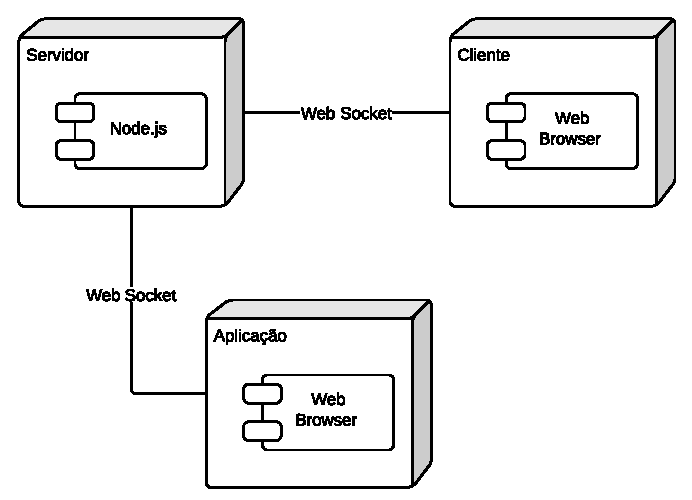
\includegraphics[scale=.5]{Components}}
\caption{Estrutura da Solução}  
\label{fig:componentes}
\end{figure}

\subsection{Tecnologias Usadas}\label{sec:lingua}

Ao longo do desenvolvimento houve a necessidade de fazer algumas escolhas a nível tecnológico, que de uma forma ou de outra tiveram influência na solução final.

Para o desenvolvimento do servidor, foi usado \textit{node.js}, facilitando o desenvolvimento de aplicações de alta escalabilidade em tempo real. Não bloqueia as chamadas de entrada e saída, e permite o suporte de diversas ligações.

Era necessário que existisse uma comunicação entre o servidor ou utilizador e a aplicação, optou-se pela biblioteca \textit{Socket.io}, em conjunto com o protocolo \textit{web sockets}. 

Ao longo da implementação foram ainda usadas algumas bibliotecas, como \textit{Prototype.js} e \textit{Swipeable}. A primeira foi escolhida por permitir a manipulação de classes e objetos baseados na mesmas. A segunda possibilitou um fácil reconhecimento dos movimentos \textit{swipe} realizados num dispositivo com propriedade \textit{touch}.

Para além das tecnologias referidas, todo o projeto foi desenvolvido com base em \textit{JavaScript}, \textit{HTML} e \textit{CSS}.

\subsection{Framework Desenvolvida} 

De modo a facilitar o desenvolvimento de aplicações para ecrãs públicos, foi desenvolvida uma \textit{framework}, que facilita a criação de controlos para as respetivas aplicações.
Esta permite a implementação de três tipos de controlo distintos, que podem ser utilizados numa vasta gama de aplicações.
Aquando do desenvolvimento o programador pode escolher qual o controlo que melhor se adapta às funcionalidades da aplicação, podendo optar por:

\begin{itemize}
\item \textbf{\textit{Joystick}}: setas de direção tradicionais;
\item \textbf{\textit{Input Text}}: caixa de introdução de texto
\item \textbf{\textit{Swipe}}: relativa aos movimentos realizados pelo toque num ecrã com propriedade \textit{touch}.
\end{itemize}

\subsection{Exemplo Implementado}

Foi desenvolvido o clássico jogo \textit{Snake}, como exemplo de aplicação interativa. 

Para que o utilizador possa usufruir do jogo é necessário que este se conecte com o ecrã. No exemplo apresentado essa ligação ocorre pela leitura de um \textit{QR code}, que se encontra sempre visível no ecrã, onde será possível jogar. Isto requer que o utilizador possua um dispositivo com ligação à Internet e uma aplicação para a leitura do \textit{QR code}.

Depois da ligação efetuada, ao longo do jogo, o utilizador poderá fazer uso dos três tipos de controlo definidos. 

Inicialmente é obrigado a inserir o seu nome, usando para isso a opção de introdução de texto. Posteriormente poderá escolher entre o \textit{joystick} ou o \textit{swipe}, servindo qualquer um deles para controlar a direção da cobra durante o jogo. 

Cabe ao utilizador a escolha do controlo adequado de acordo com as suas preferências ou facilidades. Para alterar apenas precisa de carregar no botão correspondente ao \textit{widget} desejado, na barra que aparece na parte superior do dispositivo.

Numa aplicação de cariz público, com a qual poderão interagir várias pessoas em simultâneo, é importante referir como os utilizadores são distinguidos.

Neste caso concreto, optou-se por usar a cor da cobra respetiva para escrever no ecrã os nomes acompanhados da pontuação, facilitando o reconhecimento dos próprios jogadores.

\section{Conclusões}\label{sec:conclui}

Em suma, nem tudo o que foi planeado inicialmente foi desenvolvido, contudo de um modo geral os objetivos foram alcançados. 

Houve desenvolvimento de uma \textit{framework} para facilitar a criação de controlos para aplicações públicas interativas, bem como a implementação de um exemplo prático.

Já na fase final, ainda foi possível a realização de testes, em que foi pedido a três estudantes que recorressem às funcionalidades da \textit{framework} para criarem controlos para uma aplicação à escolha. 

%%English version: comment first, uncomment second
%\bibliographystyle{unsrt-pt}  % numeric, unsorted refs
%\bibliographystyle{unsrt}  % numeric, unsorted refs
%\bibliography{refs}

\end{multicols}

\end{document}
